\chapter{Dia: 09/02/22}
\label{chap:09-02-22}

Primeiro surgiu uma tentativa de testes do dobot usando a docker porém o seguinte erro aparecia no terminal:

\begin{figure}[h!]
    \centering
    \caption{terminal}
    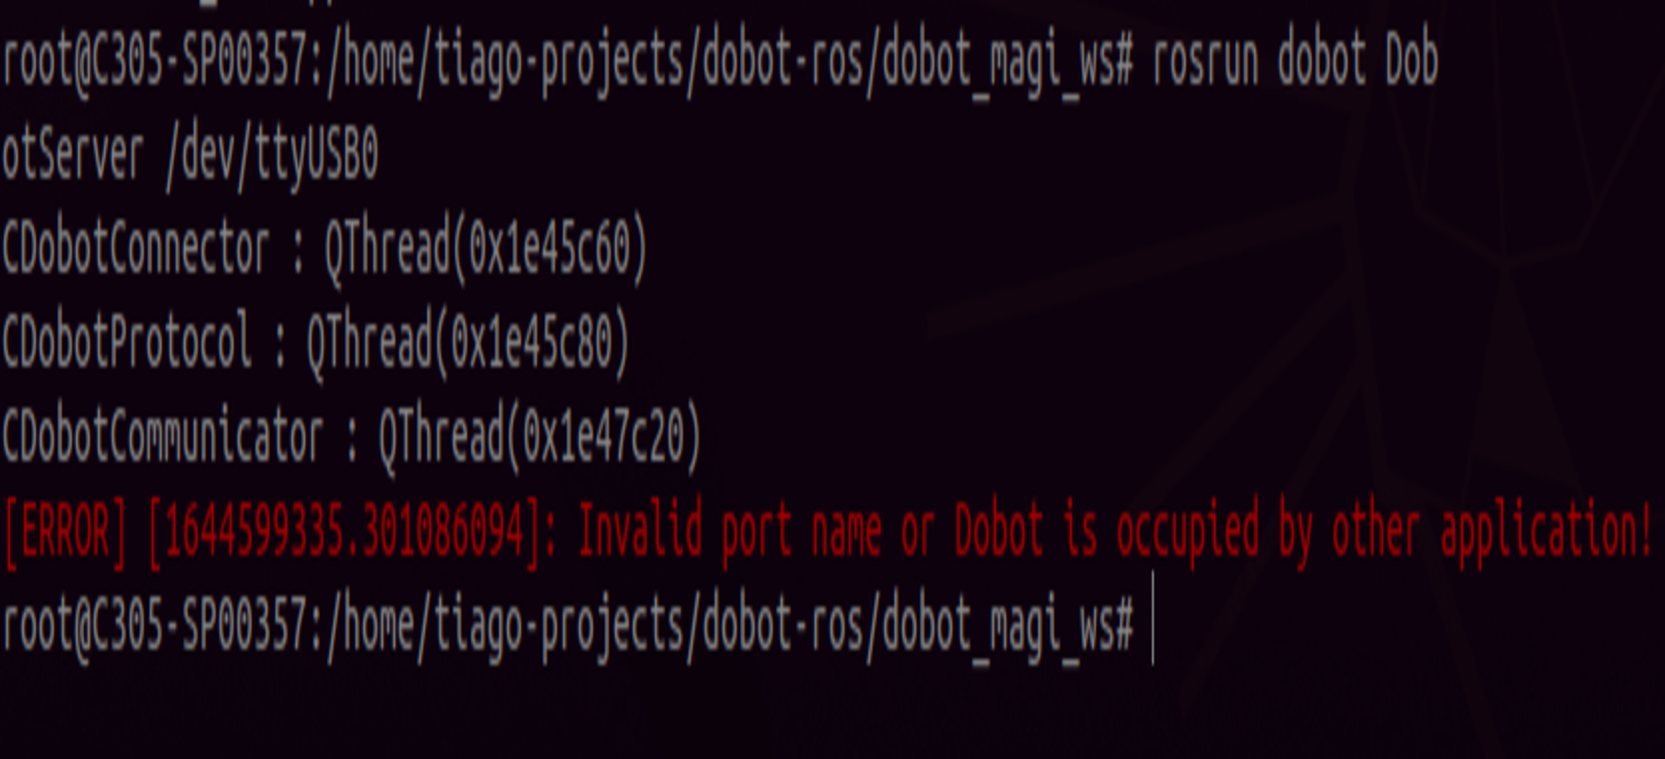
\includegraphics[width=1\textwidth]{Figures/dob1.jpg}
    \caption*{Fonte: Autoria propria.}
    \label{fig:teminal1}
\end{figure}

A primeira hipótese foi substituir a docker que estava sendo utilizada, que era uma docker de ROS Kinetic, e retorna para o tipo de docker que estava sendo utilizada anteriormente, que era uma docker de ubuntu xenial com ubuntu instalado. Isso foi feito com base no fato de que na primeira tentiva se tinha usado a docker dessa forma e tinha funcionado, precisaria de um OS para poder controlar as portas e no manual está recomendado o uso dessa versão do ubuntu com essa versão do ros instalado. A partir disso foi criado essa imagem do xenial com o ROS Kinetic instalado e armazenado no seguinte repositório no \href{https://hub.docker.com/repository/docker/tiago369/ubuntu-kinect}{DockerHUB}.

Porém, mesmo realizando isso o problema persistiu e decidiu investigar mais ainda o uso de portas USB na docker, a partir disso descobriu-se que precisava subir as portas USBs que seriam utilizadas, assim no código de docker\underline{\space}run\underline{\space}xenial.sh foi substituído a parte que sobe as portas de videos pela USB

Antes:

\begin{lstlisting}[language=Awk]
    V4L2_DEVICES=" "

    for i in {0..9}
    do
        if [ -a "/dev/ttyVideo$i" ]; then
            V4L2_DEVICES="$V4L2_DEVICES --device /dev/ttyVideo$i "
        fi
    done

    echo "V4L2_DEVICES:  $V4L2_DEVICES"
\end{lstlisting}

Depois:

\begin{lstlisting}[language=Awk]
    V4L2_DEVICES=" "

    for i in {0..9}
    do
        if [ -a "/dev/ttyUSB$i" ]; then
            V4L2_DEVICES="$V4L2_DEVICES --device /dev/ttyUSB$i "
        fi
    done

    echo "V4L2_DEVICES:  $V4L2_DEVICES"
\end{lstlisting}

Depois disso o DOBOT conseguiu se conectar e se partiu para o desenvolvimento dos códigos